\documentclass[letterpaper,12pt]{article}
\usepackage{geometry}
\usepackage{lipsum}  
\usepackage{graphicx}
\usepackage{subcaption}
\usepackage[english]{babel}
\usepackage{fancyhdr}
\usepackage{hyperref}
\usepackage{multicol}
\usepackage{float}
\usepackage{changepage}
\usepackage{booktabs}
\usepackage{cite}

\graphicspath {{figures/}}

\setlength{\headheight}{15pt}

\pagestyle{fancy}
\fancyhf{}
\lhead{\textbf{Version: 2.0}}
\rhead{\thepage}
\lfoot{Sam Penders}
\rfoot{\textit{Mu2e: University of Minnesota}}

\renewcommand{\footrulewidth}{1pt}


\begin{document}
\begin{titlepage}
	\centering
	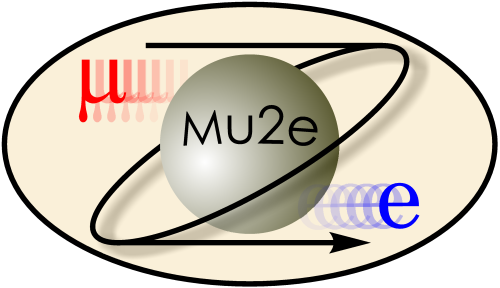
\includegraphics[width=0.5\textwidth]{mu2e_logo_oval.png}\par\vspace{2cm}
	{\scshape\LARGE Epoxying in CO$_2$ Endpieces\\ Version 2.0\par}
	\vspace{3cm}
	{\Large Sam Penders and Mitch Frand \par}
	\vspace{3cm}
	{\large University of Minnesota\par}
 	\vspace{.5cm}
	{\large June 5, 2018\par}
	% Bottom of the page
	\vfill

{\href{mailto:pende061@physics.umn.edu}
    {\tt{pende061@umn.edu}}\par} 
{\href{mailto:frand053@umn.edu}
    {\tt{frand053@umn.edu}}\par} 
\end{titlepage}

\clearpage
\setcounter{page}{2}


\section{Goal}
Epoxy plastic endpieecs with a viton hose into the ends of a pallet of straws so they may be leak tested.


\section{Equipment}
\begin{multicols}{2}
\begin{itemize}
	\item Pallet with 24 straws (paper removed)
	\item Mixing tray
	\item Cotton swabs
	\item Nitrile gloves
	\item 3M Scotch--Weld DP-190 Translucent epoxy
	\item Epoxy dispensing gun
	\item Plastic CO$_2$ endpieces ($\times 48$)
	\item $\sim$1.5'' viton hose segments ($\times 48$)
\end{itemize}
\end{multicols}


\section{Risks and Dangers}
3M DP190 epoxy routes of entry, risks, and first aid:
\begin{itemize}
\item {\bf Inhalation:} Remove the person to fresh air. If you feel unwell, seek medical attention.
\item {\bf Skin Contact:} Immediately wash affected area with soap and water. Remove contaminated clothing and wash before reuse. If symptoms develop, seek medical attention.
\item {\bf Eye Contact:} Flush with large amounts of water in eye wash station, located by the main door in PAN 464, and the door without the Ucard reader in room 450. Remove contact lenses is easy to do. If symptoms develop, seek medical attention.
\item {\bf If swallowed:} Rinse mouth. If you feel unwell, get medical attention.
\end{itemize}

\noindent
Isopropyl alchohol (propanol) routes of entry, risks, and first aid:
\begin{itemize}
\item {\bf Eyes:} Irritating, and may injure eye tissue if not removed promptly. Flush with plenty of water in eye wash station for at least 15 minutes. Seek medical attention immediately.

\item {\bf Inhalation:} Exposure to vapors may cause the following effects: Headaches. Dizziness. Central nervous system effects. Pulmonary edema. Slightly irritating to eyes and respiratory tract. Gas, vapor, mist, or dust concentrations may be harmful if inhaled. High concentrations may be fatal. If inhaled, remove from exposure. Administer artificial respiration if not breathing. Keep warm and quiet. Get medical attention immediately.

\item {\bf Ingestion:} May cause chemical pneumonitis if aspirated into lungs. Single dose toxicity is low. If ingested, do not induce vomiting. Keep calm. Contact physician or poison control center immediately.

\item {\bf Skin:} Frequent or prolonged contact may irritate the skin and cause a skin rash (dermatitis). Flush skin with water and follow by washing skin with soap and water. Remove
contaminated clothing and footwear.

\end{itemize}

\section{Procedure}
\begin{enumerate}
\item Put on nitrile gloves. \label{first}

\item Unscrew the plastic track that holds the ends of the straws on one side of the pallet. Slide this towards the center of the pallet so that the straws hand off of the tracks by about a half inch on either end.

\item Insert the barbed end of CO$_2$ into an approximately $1.5$ inch piece of viton hose.
%
\item Clear any dried epoxy from the end of the epoxy tube. With the epoxy tube loaded into the epoxy gun, pull the trigger of the epoxy gun until a small amount of both the resin and curing agent come out, into the garbage. Now dispense a small amount (about the size of a quarter) of resin and epoxy into a mixing dish, making sure the two substances come out in approximately equal amounts.
%
\item Vigorously stir the resin and curing agent together in the dish with the wooden end of the cotton swab, for about 2 minutes. Make sure the edges of the epoxy are mixed well. The mixed substance should look uniform. Throw away the mixing stick.
%
\item Gather a rice-sized amount of epoxy onto the wooden end of a cotton swab. Spread this evenly onto the outside of the plastic endpiece, avoiding getting any on the inside part.
%
\item While very gently holding the end of a straw against the plastic track on the pallet, insert the endpiece into the end of a straw while slowly twisting the endpiece to evenly distribute the epoxy onto the straw. Some excess epoxy should have been forced out of the straw, which indicates a good seal. Wipe this off with the swab end of a stick. \label{last}
%
\item Repeat steps \ref{first}--\ref{last} for each straw end. One person may work on each side, working in opposite directions.
\end{enumerate}

\newpage
\section{Troubleshooting}
\begin{itemize}
\item {\bf Problem:} The straw end is slightly crumpled so the endpiece will not go in.
		\begin{adjustwidth}{1cm}{}
		{\bf Solution:} Using the small scissors, evenly trim off about 5 mm of the straw end to remove the problematic section. Try again to insert the endpiece.
		\end{adjustwidth}
		
\item {\bf Problem:} The straws are too short to epoxy in endpieces; the plastic track gets in the way.
		\begin{adjustwidth}{1cm}{}
		{\bf Solution:} Epoxying in endpieces while the straw end is less that a half inch from the plastic tracks poses a major risk of epoxying the straw to the track itself. Use a screwdriver to carefully remove the screws on one of the plastic tracks. Slide the plastic track an inch or so towards the center of the pallet so it is no longer in the way. 
		\end{adjustwidth}
		
\item {\bf Problem:} I got epoxy on the straw and/or pallet.
		\begin{adjustwidth}{1cm}{}
		{\bf Solution:} Dispense a small amount of isopropyl alcohol into a mixing dish. Soak a clean cotton swab in the alcohol and clean the epoxy off of the affected area. Wipe off any excess alcohol with a dry cotton swab.
		\end{adjustwidth}			
		
\end{itemize}



\end{document}